\documentclass[11pt,aspectratio=169,hyperref={colorlinks}]{beamer}

\usetheme{Singapore}

\usecolortheme[snowy]{owl}

\usepackage[utf8]{inputenc}
\usepackage[T1]{fontenc}
\usepackage[american]{babel}
\usepackage{graphicx}
\usepackage{hyperref}
\hypersetup{
    colorlinks=true,
    urlcolor=[rgb]{0,0,0.61},
    linkcolor=[rgb]{0,0,0.61}}
 
    
%\usepackage[natbib=true,style=authoryear,backend=bibtex,useprefix=true]{biblatex}
\usepackage{blindtext}
\usepackage[natbib=true,style=numeric,backend=bibtex,useprefix=true]{biblatex}
\setbeamertemplate{bibliography item}{\insertbiblabel}
\setbeamerfont{caption}{size=\footnotesize}
\setbeamertemplate{frametitle continuation}{}

\setcounter{tocdepth}{1}
\renewcommand*{\bibfont}{\scriptsize}
\addbibresource{lecture_2.bib}

\renewcommand*{\thefootnote}{\fnsymbol{footnote}}

\usenavigationsymbolstemplate{}
\setbeamertemplate{footline}{%
    \raisebox{5pt}{\makebox{\hfill\makebox[20pt]{\color{gray}
          \scriptsize\insertframenumber}}}\hspace*{5pt}}

\usepackage{epigraph}
% \epigraphsize{\small}% Default
\setlength\epigraphwidth{14cm}
\setlength\epigraphrule{0pt}
\usepackage{etoolbox}
\makeatletter
\patchcmd{\epigraph}{\@epitext{#1}}{\itshape\@epitext{#1}}{}{}
\makeatother

%-------------------------------------------------------------------------------

\usepackage{mathtools}
\usepackage{xcolor}
\usepackage{soul}
\newcommand{\mathcolorbox}[2]{\colorbox{#1}{$\displaystyle #2$}}

%-------------------------------------------------------------------------------

% OwlGreen - customized to make the header violet color
\definecolor{OwlGreen}{RGB}{51,0,102}
\definecolor{magenta}{RGB}{248,206,204}
\definecolor{fuschia}{RGB}{255,0,255}
\definecolor{blue}{RGB}{0,0,156}


\usepackage{xcolor, soul}
\sethlcolor{magenta}

%-------------------------------------------------------------------------------

\setbeamertemplate{bibliography item}{}
\renewcommand*{\bibfont}{\scriptsize}
\addbibresource{main.bib}

\setbeamerfont{caption}{size=\footnotesize}
\setbeamertemplate{frametitle continuation}{}
\setcounter{tocdepth}{1}

%-------------------------------------------------------------------------------

\usenavigationsymbolstemplate{}
\setbeamertemplate{footline}{%
    \raisebox{5pt}{\makebox{\hfill\makebox[20pt]{\color{gray}
          \scriptsize\insertframenumber}}}\hspace*{5pt}}

\renewcommand*{\thefootnote}{\fnsymbol{footnote}}

%-------------------------------------------------------------------------------

\usepackage[natbib=true,style=numeric,backend=bibtex,useprefix=true]{biblatex}

%\definecolor{OwlGreen}{RGB}{75,0,130} % easier to see
\setbeamertemplate{bibliography item}{\insertbiblabel}
\setbeamerfont{caption}{size=\footnotesize}
\setbeamertemplate{frametitle continuation}{}

\setcounter{tocdepth}{1}
\renewcommand*{\bibfont}{\scriptsize}
\addbibresource{lecture_2_DRAFT.bib}

\renewcommand*{\thefootnote}{\fnsymbol{footnote}}

\usenavigationsymbolstemplate{}
\setbeamertemplate{footline}{%
    \raisebox{5pt}{\makebox{\hfill\makebox[20pt]{\color{gray}
          \scriptsize\insertframenumber}}}\hspace*{5pt}}

\usepackage{epigraph}
% \epigraphsize{\small}% Default
\setlength\epigraphwidth{14cm}
\setlength\epigraphrule{0pt}
\usepackage{etoolbox}
\makeatletter
\patchcmd{\epigraph}{\@epitext{#1}}{\itshape\@epitext{#1}}{}{}
\makeatother


\author{Patrick Hall}
\title{Responsible Machine Learning\footnote{\tiny{This material is shared under a \href{https://creativecommons.org/licenses/by/4.0/deed.ast}{CC By 4.0 license} which allows for editing and redistribution, even for commercial purposes. However, any derivative work should attribute the author.}}}
\subtitle{Lecture 2:  Post-hoc Explanations}
\institute{The George Washington University}
\date{\today}



\begin{document}
	
	\maketitle
	
	\begin{frame}
	
		\frametitle{Contents}
		
		\tableofcontents{}
		
	\end{frame}

\renewcommand*{\thefootnote}{\arabic{footnote}}

%-------------------------------------------------------------------------------
	\section{Introduction}
%-------------------------------------------------------------------------------

	
		\subsection*{} %just for progress indicator
			
		\begin{frame}
		
			\frametitle{A Responsible Machine Learning Workflow\footnote{\href{https://www.mdpi.com/2078-2489/11/3/137/htm}{\textit{A Responsible Machine Learning Workflow}}}}
			
			\begin{figure}[htb]
				\begin{center}
					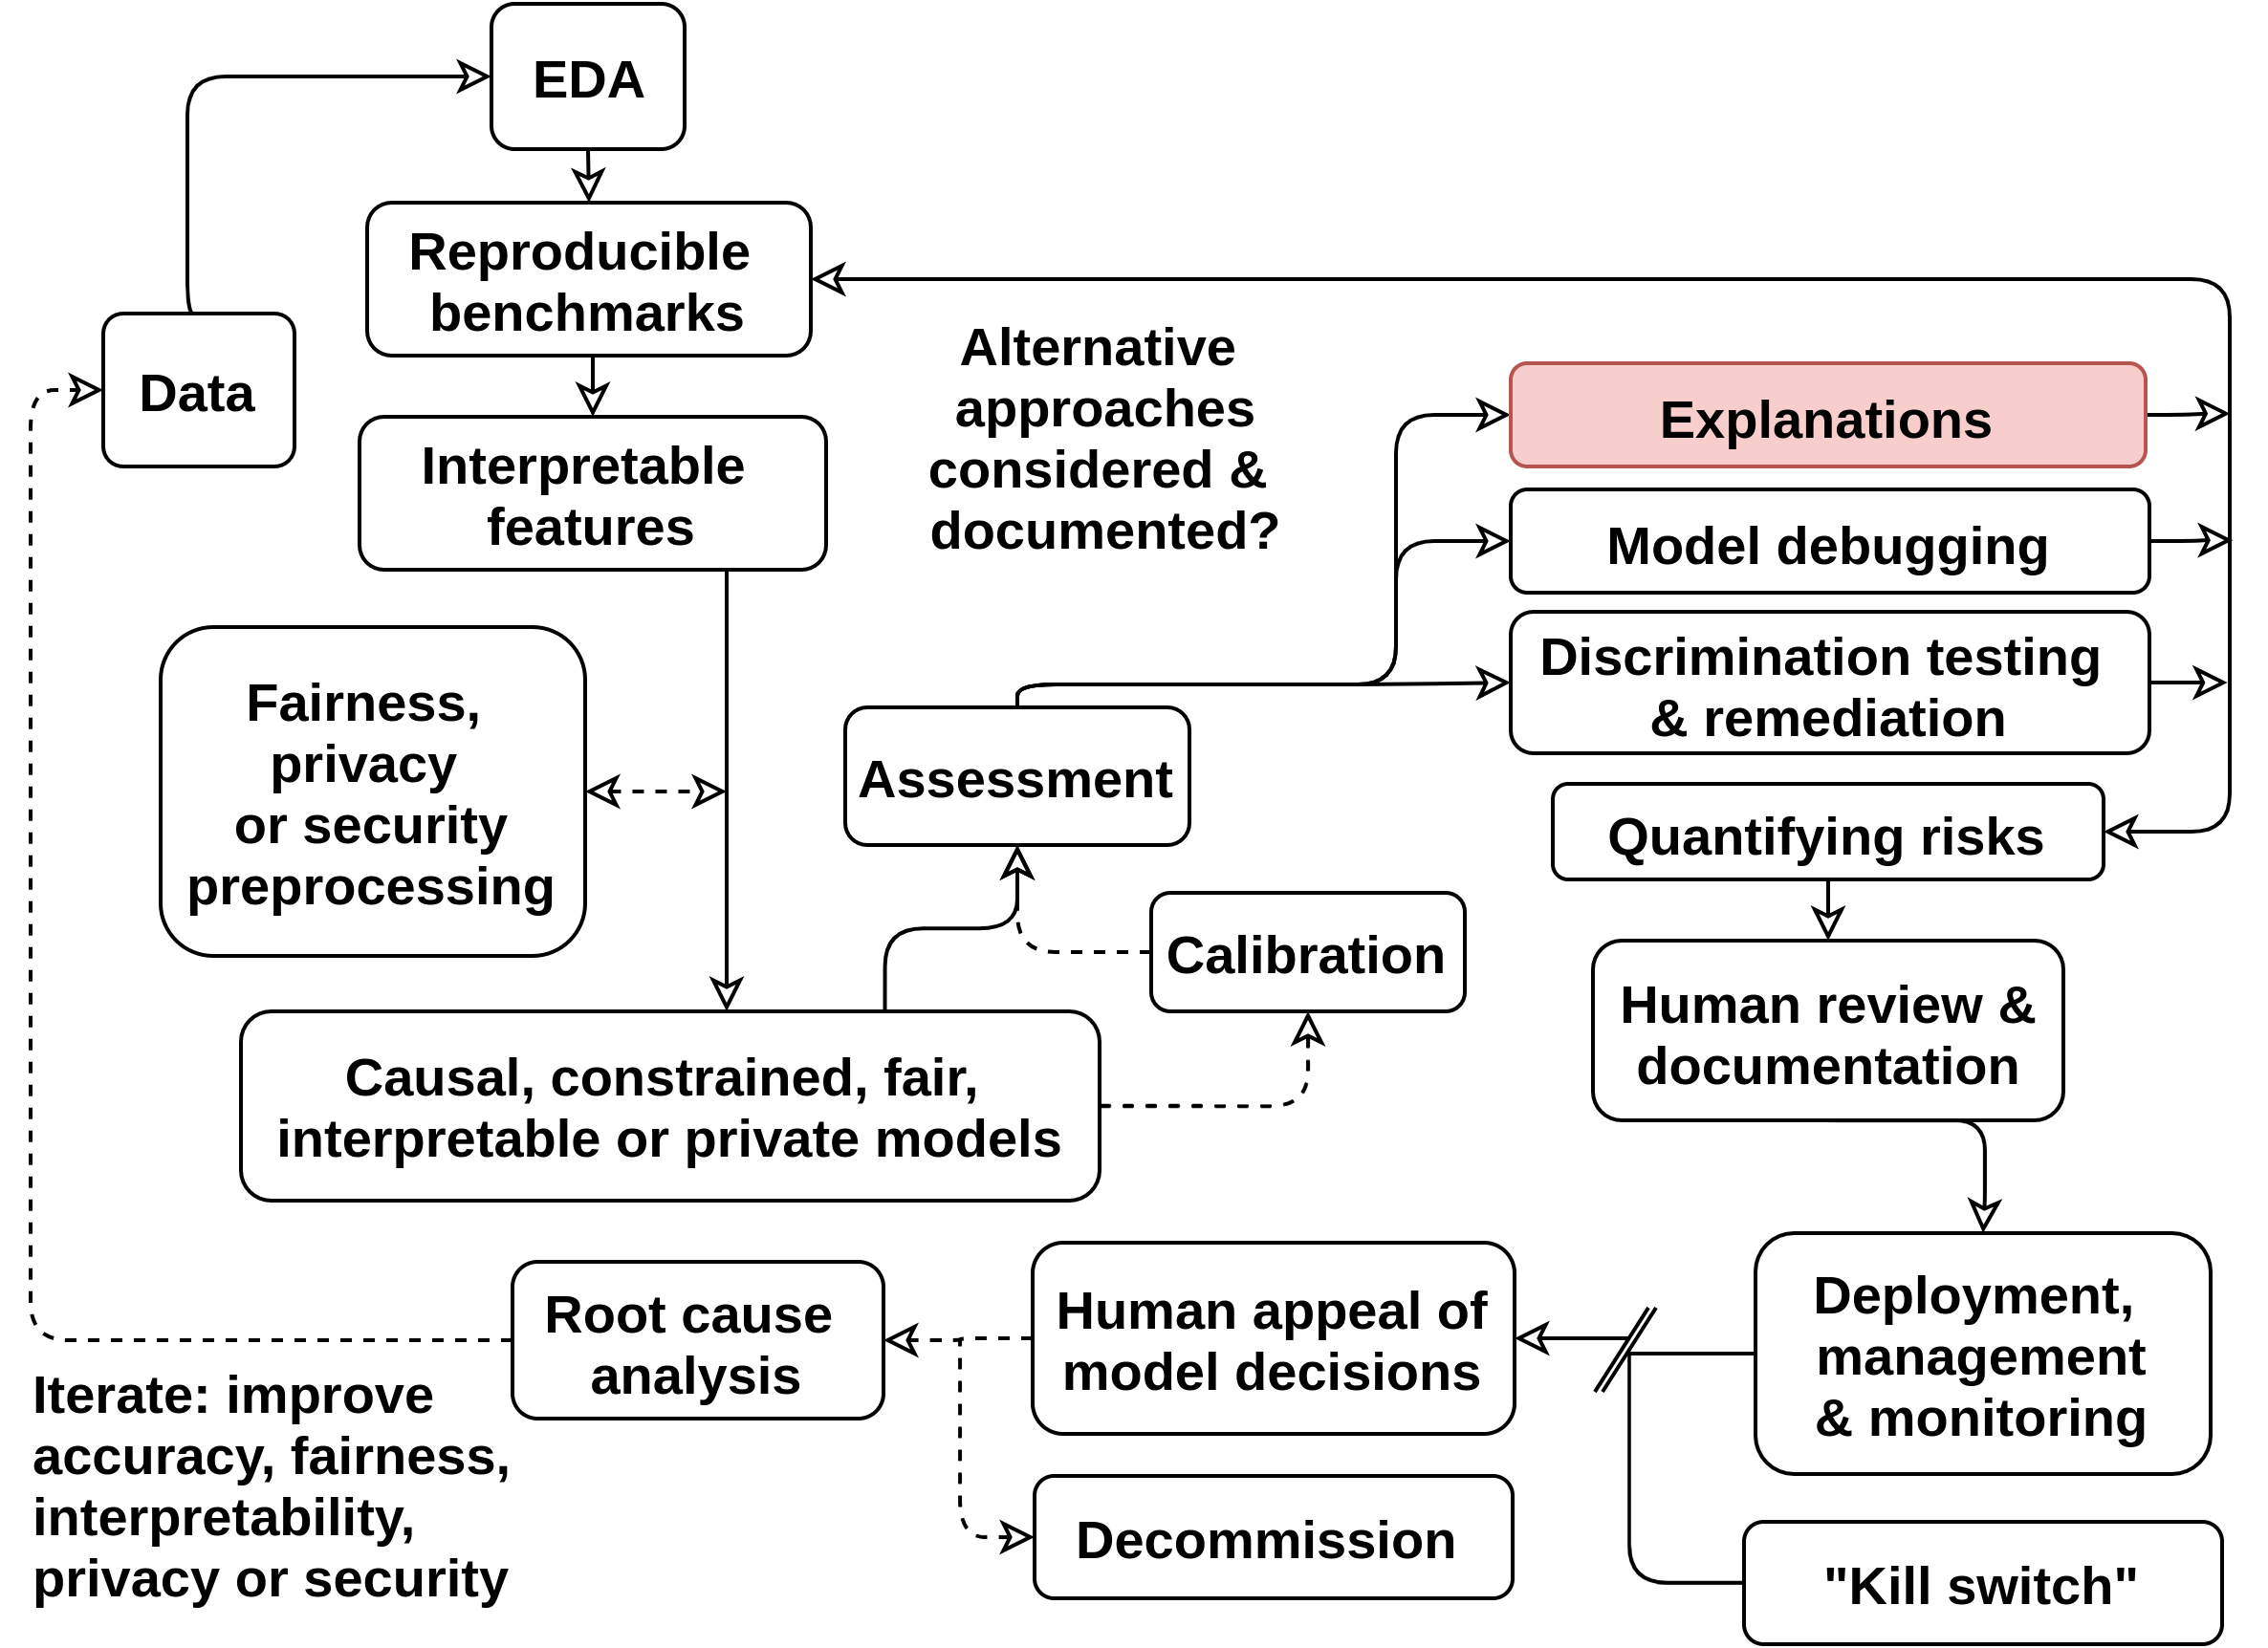
\includegraphics[height=150pt]{../img/rml_diagram_lec2_hilite.png}
					\label{fig:blueprint}
				\end{center}
			\end{figure}		
					
		\end{frame}					


		\begin{frame}[allowframebreaks]
			
			\frametitle{Lecture 2 Agenda}
 
			\begin{itemize}
				\item{Overview of Explainable ML}
				\item{Understanding and Trust}
				\item{The Dark Side}
				\item{Surrogates}
				\item{High Stakes Applications}
			\end{itemize}
				
		\end{frame}


	\begin{frame}[t]
		
		\frametitle{What is an Explanation in Machine Learning (ML)?}
		
		\epigraph{“A collection of visual and/or interactive artifacts that provide a user with sufficient description of the model behavior to accurately perform tasks like evaluation, trusting, predicting, or improving the model.”}{--- \textup{Sameer Singh}, UCI}		
		
		\scriptsize Variously defined along with aliases or similar concepts:
		\begin{itemize}\scriptsize
			\item ``Towards a Rigorous Science of Interpretable Machine Learning'' (\citet{been_kim1})
			\item ``Explaining Explanations'' (\citet{gilpin2018explaining})
			\item ``A Survey Of Methods For Explaining Black Box Models'' (\citet{guidotti2018survey})
			\item ``The Mythos of Model Interpretability'' (\citet{lipton1})
		 	\item \textit{Interpretable Machine Learning} (\citet{molnar})
			\item ``Interpretable Machine Learning: Definitions, Methods, and Applications'' (\citet{murdoch2019interpretable})
			\item ``Challenges for Transparency'' (\citet{weller2017challenges}). 
		\end{itemize}\normalsize
		
	\end{frame}
	
	\begin{frame}
	
		\frametitle{What do \textit{\textbf{I}} Mean by Explainable ML?}

		Mostly post-hoc techniques used to enhance \textit{\textbf{understanding}} of trained model mechansims and predictions, e.g. ...
		\begin{itemize}
			\item \textbf{Direct measures of global and local feature importance}: 
			\begin{itemize}\footnotesize
				\item Gradient-based feature attribution (\citet{grad_attr})
				\item Shapley values (\citet{shapley}, \citet{shapley1953value})
			\end{itemize}
			\item \textbf{Global and local surrogate models}: 
			\begin{itemize}\footnotesize
				\item Decision tree variants (\citet{viper}, \citet{dt_surrogate1})
				\item Anchors (\citet{anchors})
				\item Local interpretable model-agnostic explanations (LIME) (\citet{lime})
			\end{itemize}
			\item \textbf{Global and local visualizations of trained model predictions}: 
			\begin{itemize}\footnotesize
				\item Accumulated local effects (ALE) (\citet{ale_plot}) 
				\item Partial dependence (\citet{esl})
				\item Individual conditional expectation (ICE) (\citet{ice_plots})
			\end{itemize}
		\end{itemize}\normalsize
			
	\end{frame}

	\begin{frame}
	
		\frametitle{Why Explainable ML?}
		
		Responsible Use of Explainable ML can enable:
		\begin{itemize}
			\item Human learning from machine learning
			\item Human appeal of automated decisions
			\item Regulatory compliance\footnote{\tiny{In the U.S., interpretable models, explanations, and the model documentation they enable may be required under the Civil Rights Acts of 1964 and 1991, the Americans with Disabilities Act, the Genetic Information Nondiscrimination Act, the Health Insurance Portability and Accountability Act, the Equal Credit Opportunity Act, the Fair Credit Reporting Act, the Fair Housing Act, Federal Reserve SR 11-7, and the European Union (EU) Greater Data Privacy Regulation (GDPR) Article 22 \cite{ff_interpretability}.}}
			\item White-hat hacking and security audits of ML models
		\end{itemize}
		\vspace{10pt}
		Even logistic regression is often ``explained'',  or post-processed, for credit scoring, e.g. max. points lost method and adverse action notices.

	\end{frame}

	\begin{frame}[t]
	
		\frametitle{Why Propose Guidelines?}		

		Misuse and Abuse of Explainable ML can enable:
		\begin{itemize}\footnotesize
			\item Model and data stealing (\citet{model_stealing}, \citet{membership_inference}, \citet{shokri2019privacy})
			\item False justification for harmful black-boxes, e.g. ``fairwashing'' (\citet{fair_washing}, \citet{please_stop})
		\end{itemize}
		\vspace{5pt}		
		Explainable ML is already in-use: 
		\begin{itemize}\footnotesize
		\item Numerous open source\footnote{\tiny{\textcolor{magenta}{Please contribute:} \url{https://github.com/jphall663/awesome-machine-learning-interpretability}.}} and commercial packages\footnote{\tiny{For instance Datarobot, H2O Driverless AI, SAS Visual Data Mining and Machine Learning, Zest AutoML.}} are available today.
		\item At least gradient-based feature attribution, partial dependence, and surrogate models are used for model validation in financial services today.\footnote{\tiny{See: \url{https://ww2.amstat.org/meetings/jsm/2019/onlineprogram/AbstractDetails.cfm?abstractid=303053}.}}\textsuperscript{,}\footnote{\tiny{See: Working paper: ``SR 11-7, Validation and Machine Learning Models'', Tony Yang, CFA, CPA, FRM. KPMG USA. \label{fn:yang}}} 
		\end{itemize}
		\vspace{5pt}	
		Regulatory guidance is not agreed upon yet.\footnote{\tiny{See: \url{https://www.americanbanker.com/news/regulators-must-issue-ai-guidance-or-fdic-will-mcwilliams}.}}
		\normalsize	
		
	\end{frame}

	\begin{frame}
	
		\frametitle{Guidelines for Responsible Use of Explainable ML}
		
		\begin{enumerate}\Large
			\item \textbf{Use explainable ML to enhance understanding.}
			\item \textbf{Learn how explainable ML is used for nefarious purposes.}
			\item \textbf{Augment surrogate models with direct explanations.}
			\item \textbf{Use highly transparent mechanisms for high stakes applications (\citet{please_stop}).}
		\end{enumerate}
		
	\end{frame}

%-------------------------------------------------------------------------------
	\section{Understanding and Trust}
%-------------------------------------------------------------------------------

	\subsection*{} % just for progress indicator

	\begin{frame}
	
		\frametitle{1: Use Explainable ML to \textbf{Enhance Understanding}}
		
		\begin{itemize}\Large
			\item{Explanations enhance understanding \textbf{directly}, and increase trust as a \textbf{side-effect}.}
			\vspace{10pt}
			\item{Models can be \textbf{understood and not trusted}, and \textbf{trusted but not understood}.}
			\vspace{10pt}
			\item{Explanations \textbf{alone} are neither necessary nor sufficient for trust.}
			\vspace{10pt}
			\item{Good explanations \textbf{enable human appeal} of model decisions.}
		\end{itemize}
		
	\end{frame}

	\begin{frame}[label={no_trust}]
	
		\frametitle{Understanding Without Trust}
		
					\begin{columns}
				
						\column{0.5\linewidth}
						\centering
						\vspace{7pt}\\
						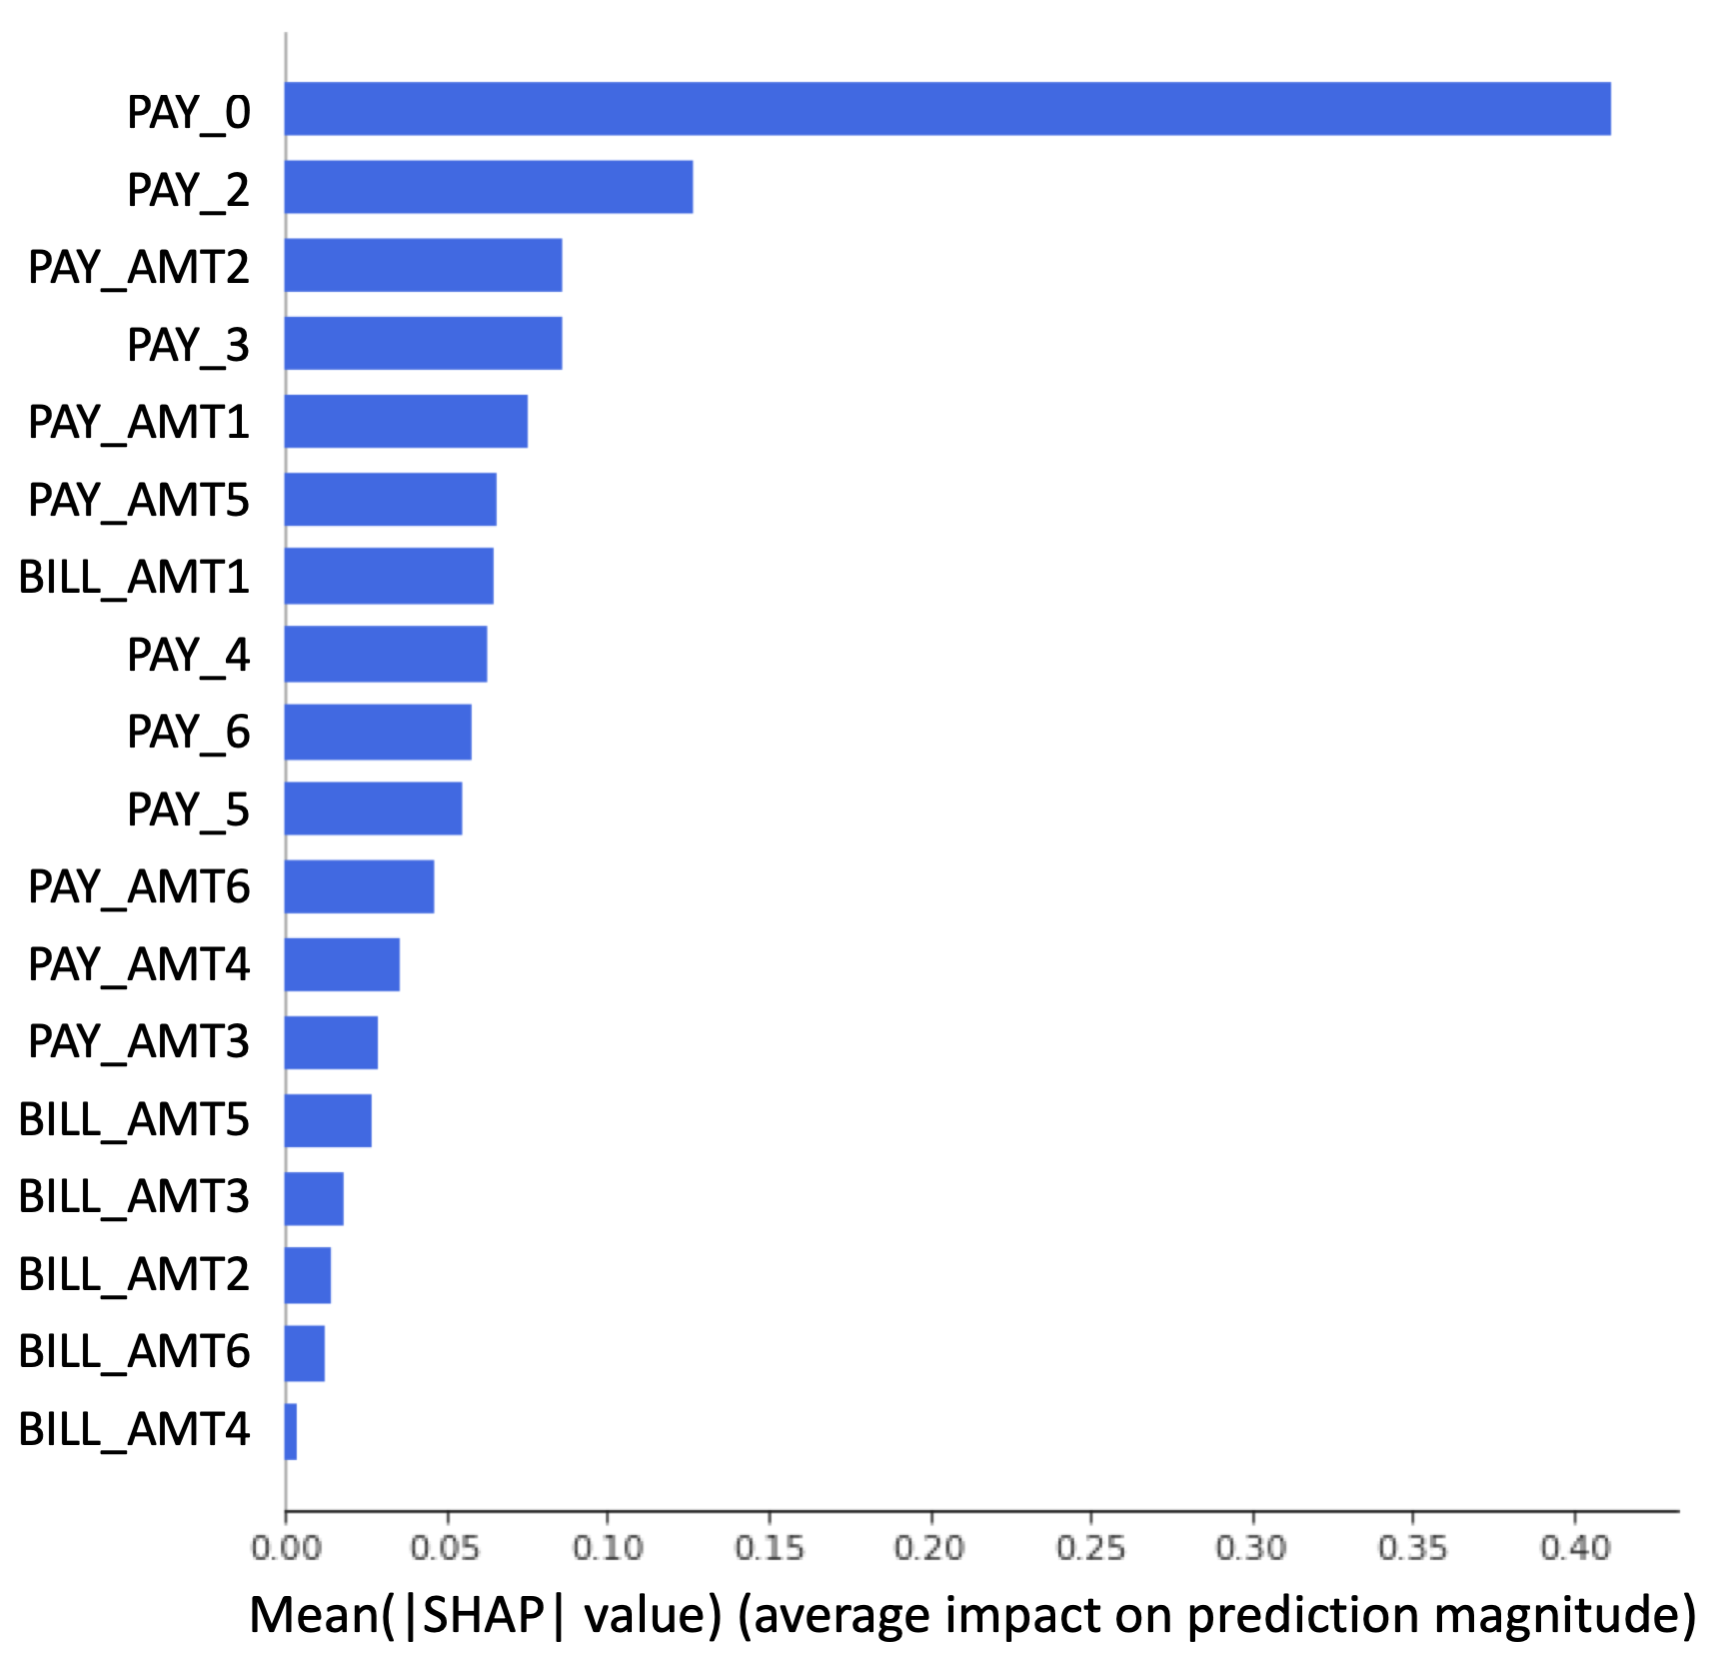
\includegraphics[height=140pt]{../img/global_shap.png}\\
						\vspace{5pt}
						\tiny{$g_{\text{mono}}$ monotonically-constrained probability of default (PD) classifier trained on the UCI credit card dataset over-emphasizes the most important feature, a customer's most recent repayment status, $\text{PAY\_0}$ \cite{uci}.}

						\vspace{10pt}
						\column{0.6\linewidth}
						\centering
						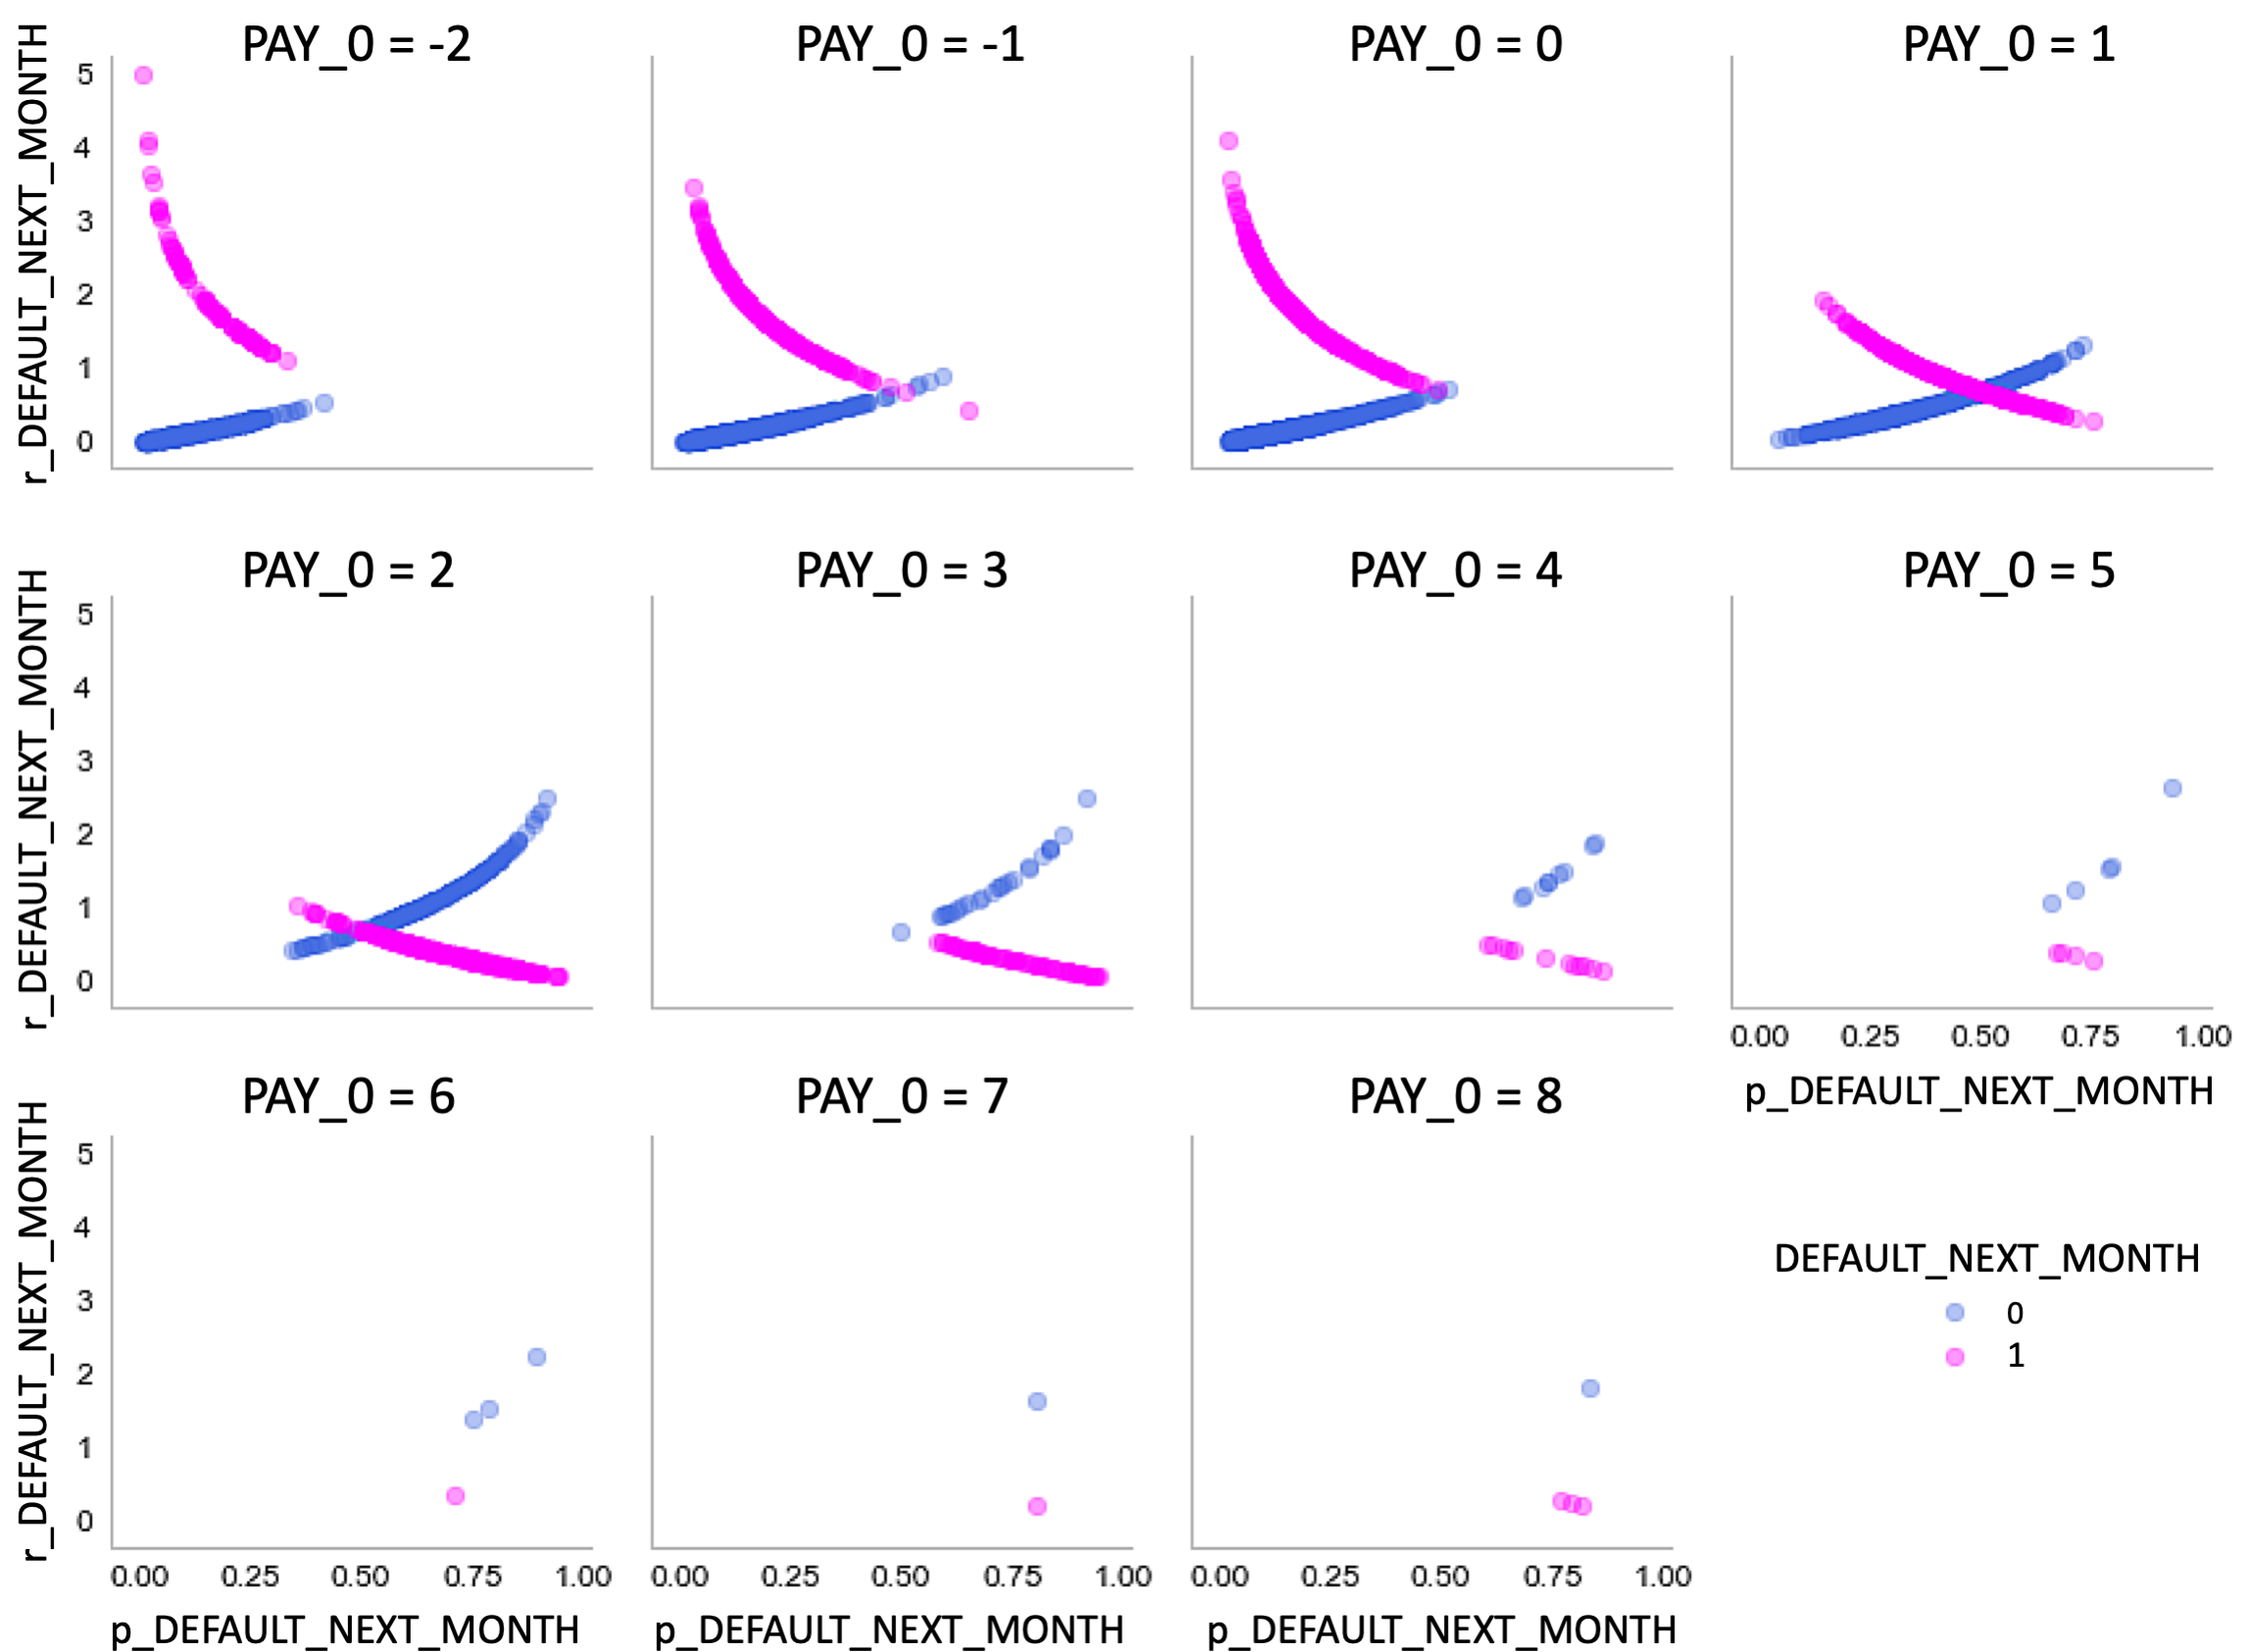
\includegraphics[height=130pt]{../img/resid.png}\\
						\vspace{5pt}
						\tiny{$g_{\text{mono}}$ also struggles to predict default for favorable statuses, $-2  \leq \texttt{PAY\_0}  < 2$, and often cannot predict on-time payment when recent payments are late, $\text{PAY\_0} \geq 2$}.
				
					\end{columns}
					\normalsize				
		
	\end{frame}
	
	\begin{frame}
	
		\frametitle{Trust Without Understanding}
		\Large
		Years before reliable explanation techniques were widely acknowledged and available, black-box predictive models, such as autoencoder and MLP neural networks, were used for fraud detection in the financial services industry (\citet{gopinathan1998fraud}). When these models performed well, they were trusted.\footnote{\tiny{For example: \url{https://www.sas.com/en_ph/customers/hsbc.html}, \url{https://www.kdnuggets.com/2011/03/sas-patent-fraud-detection.html}}.} However, they were not explainable or well-understood by contemporary standards.  

	\end{frame}


%-------------------------------------------------------------------------------
	\section{The Dark Side}
%-------------------------------------------------------------------------------

	\subsection*{} % just for progress indicator

	\begin{frame}
	
		\frametitle{2: Explainable ML Can be Used for \textbf{Nefarious Purposes}}	
		\Large
		When unintentionally misused, explainable ML can act as a faulty safeguard for potentially harmful black-boxes.\\
		\vspace{10pt}
		When intentionally abused, explainable ML can be used for: 
		\begin{itemize}
			\item Stealing data, models, or other intellectual property.
			\item \textit{Fairwashing}, to mask the sociological biases of a discriminatory black-box.
		\end{itemize}
	
	\end{frame}

	\begin{frame}
	
		\frametitle{\textit{\textbf{AI Incident}}: ML Hacking}
		
\footnotesize{Many ML hacks use, or are exacerbated by, explainable ML techniques.}\footnote{\tiny{See \url{https://github.com/jphall663/secure_ML_ideas} for full size image and more information.}}
				\begin{figure}
					\begin{center}
						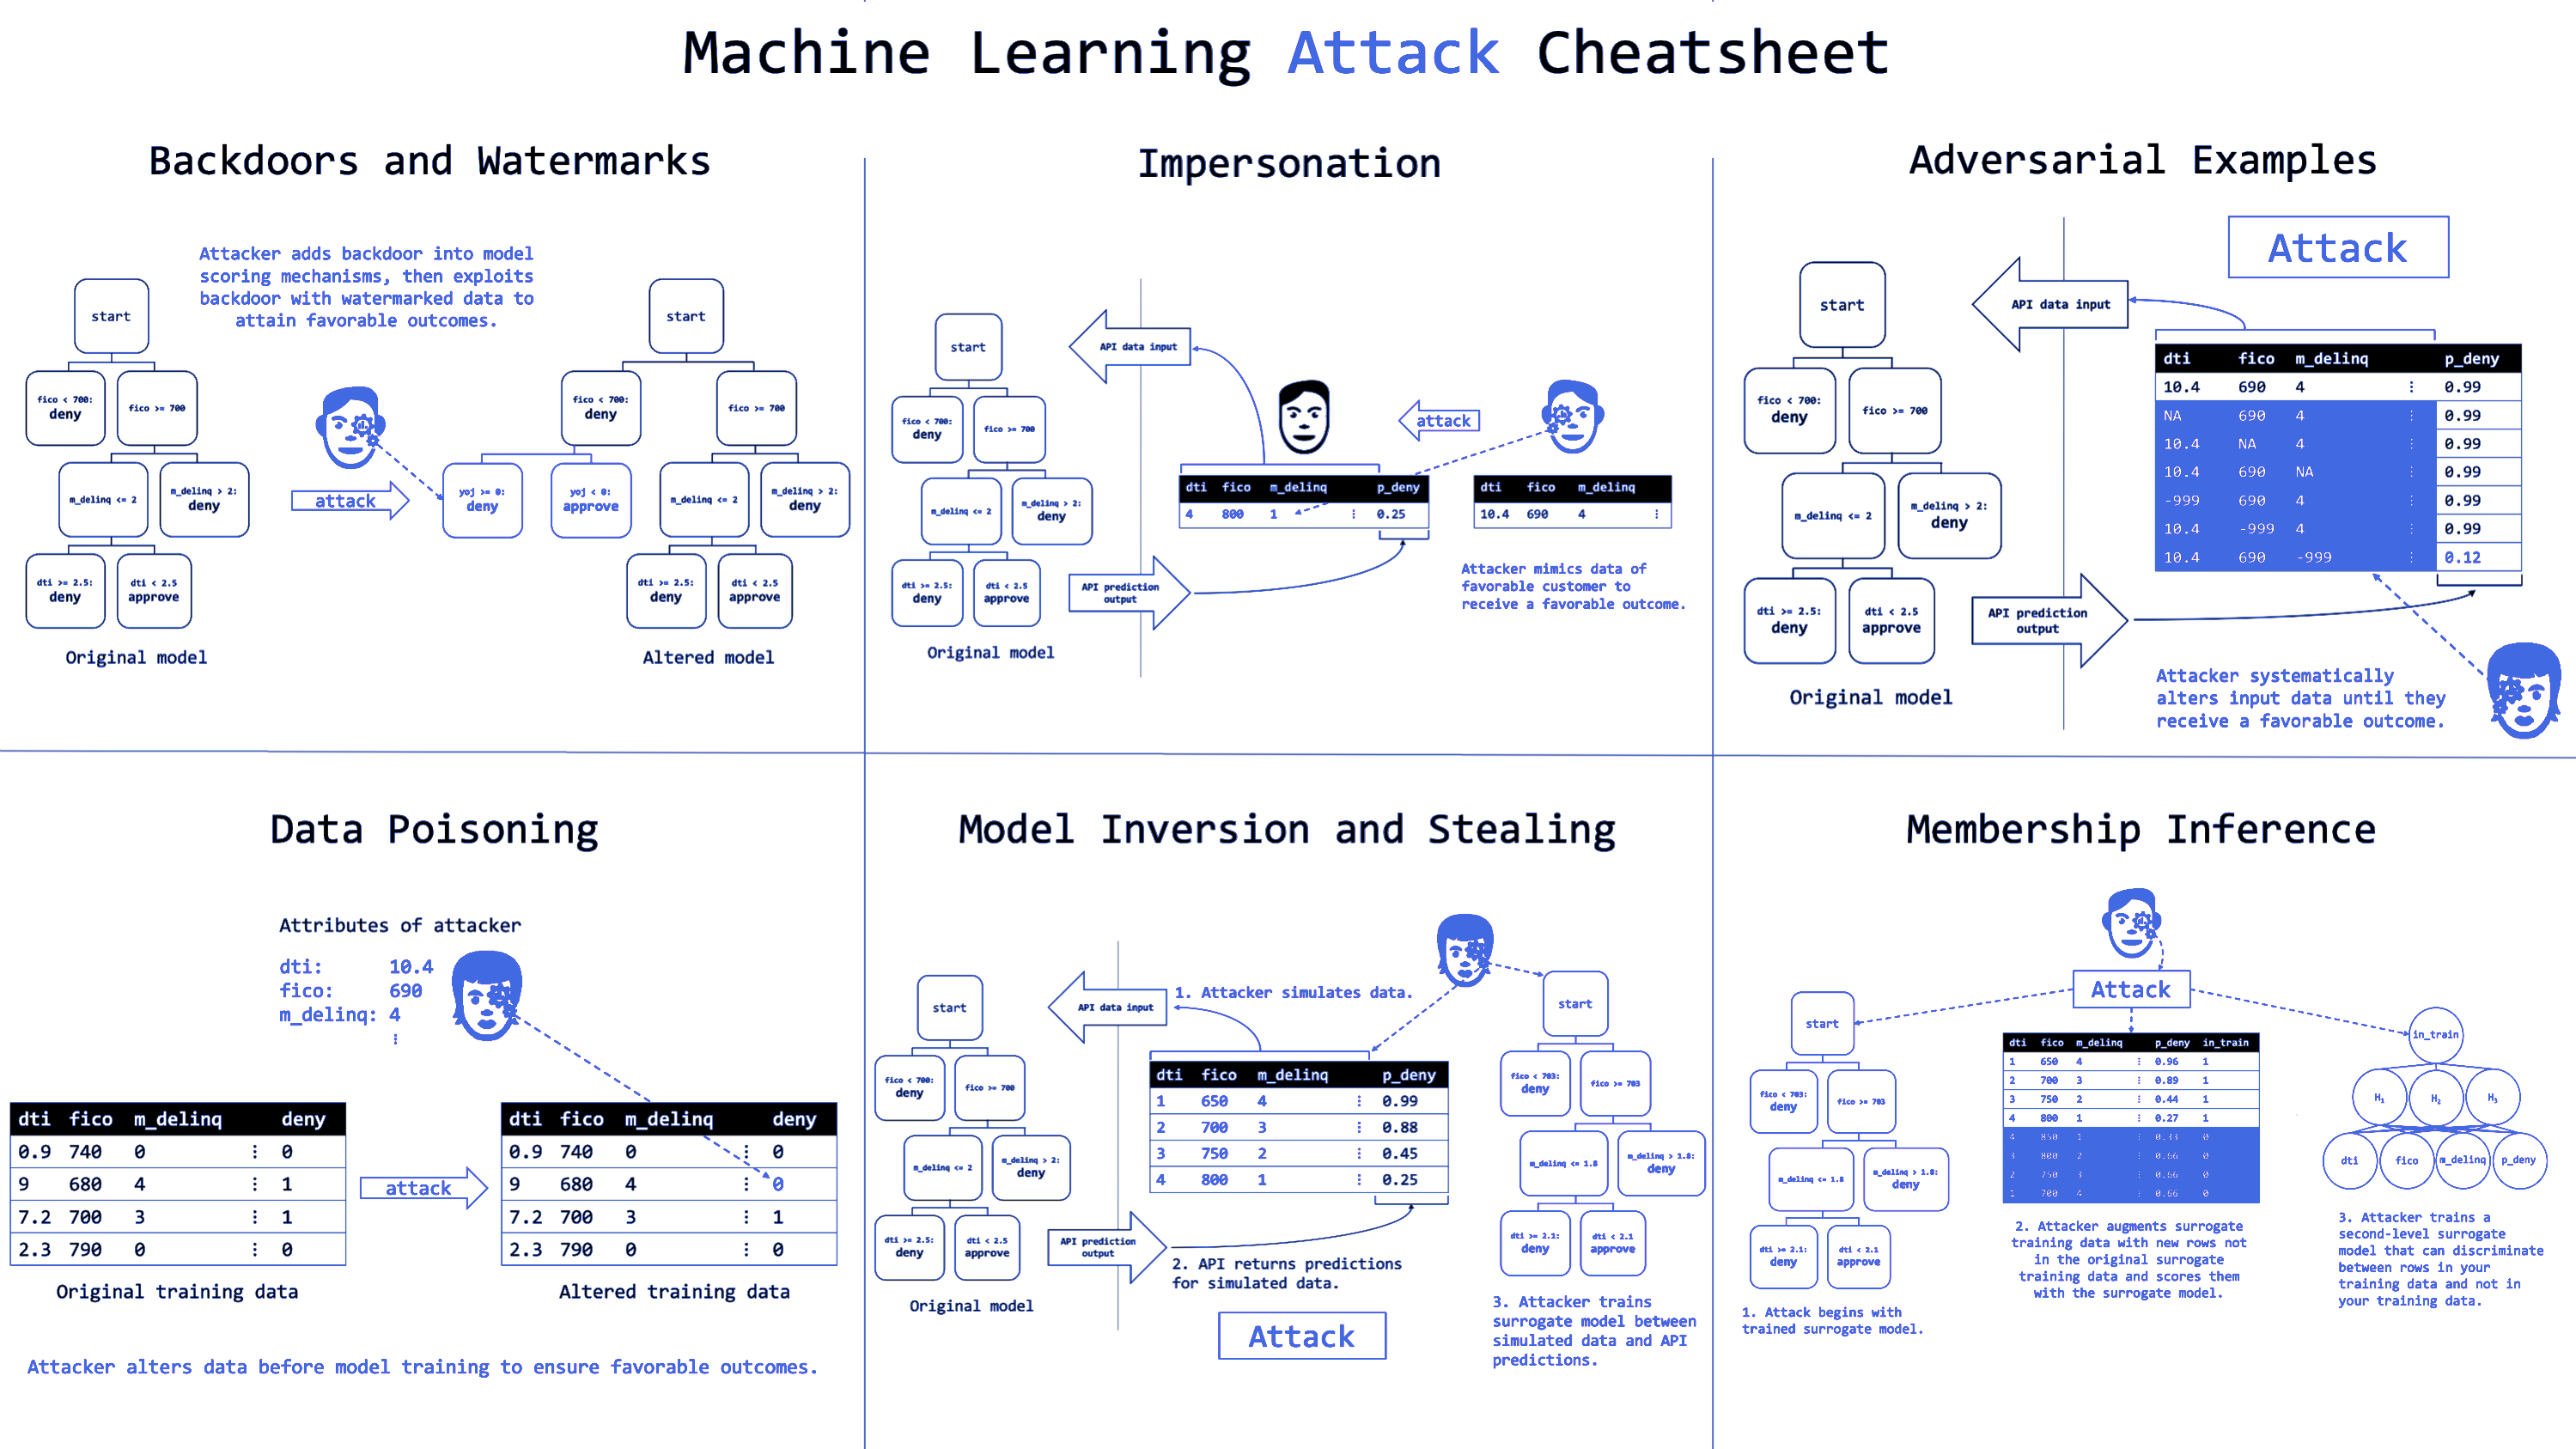
\includegraphics[height=160pt]{../img/cheatsheet_blue.png}
					\end{center}
				\end{figure}	
				\normalsize
	
	\end{frame}
	
	\begin{frame}
	
		\frametitle{\large{\textbf{Case 2.1}: White-hat Attacks Can Crack Potentially Harmful Black-boxes}}
		\large
		The flip-side of the dark side is community oversight of black-boxes.\\
		\vspace{10pt}
		Recent high profile analyses of commercial black-boxes, e.g. ... 
		\begin{itemize}		
			\item \href{https://www.propublica.org/article/machine-bias-risk-assessments-in-criminal-sentencing}{Propublica and COMPAS} (\citet{angwin16})\footnote{\tiny{This presentation makes no claim on the quality of the analysis in Angwin et al. (2016), which has been criticized, but is simply stating that such cracking is possible \cite{angwin16,}, \cite{flores2016false}}.}
			\item \href{https://medium.com/@Joy.Buolamwini/response-racial-and-gender-bias-in-amazon-rekognition-commercial-ai-system-for-analyzing-faces-a289222eeced}{Gendershades and Rekognition} (\citet{gender_shades}, \citet{raji2019actionable})
		\end{itemize}
		... \textbf{could} be characterized as white-hat attacks on proprietary black-boxes (respectively, model stealing and adversarial examples).

	\end{frame}
	
	\begin{frame}[label={not_frontline}]
	
		\frametitle{\textbf{Case 2.2}: Explanation \textbf{\textit{is Not}} a Front Line Fairness Tool}
		\large
		Use fairness tools, e.g. ...
		\vspace{5pt}
		\begin{itemize}\normalsize
			\item Disparate impact testing (\citet{feldman2015certifying})
			\item Reweighing (\citet{kamiran2012data})
			\item Reject option based classification (\citet{kamiran2012decision})
			\item Adversarial de-biasing (\citet{zhang2018mitigating})
			\item \href{https://github.com/dssg/aequitas}{aequitas}, \href{https://github.com/IBM/AIF360}{AIF360}, \href{https://github.com/LASER-UMASS/Themis}{Themis}, \href{https://github.com/cosmicBboy/themis-ml}{themis-ml}
		\end{itemize}
		\vspace{5pt}
		... for fairness tasks: bias testing, bias remediation, and to establish trust.\\
		\vspace{10pt}
		Explanations can be used to understand and augment such results.
		
	\end{frame}
	
%-------------------------------------------------------------------------------
	\section{Surrogates}
%-------------------------------------------------------------------------------

	\subsection*{} % just for progress indicator

	\begin{frame}
	
		\frametitle{What are Surrogate Models?}
		\begin{itemize}\large
			\item{Models of models (i.e. surrogate models, compressed models, extracted models) can be helpful explanatory or modeling tools, but they can also be approximate, low-fidelity explainers.}
			\vspace{10pt}
			\item{Much work in explainable ML has been directed toward improving the fidelity and usefulness of surrogate models (e.g., \citet{dt_surrogate2}, \citet{viper}, \citet{dt_surrogate1}, \citet{lime-sup}, \citet{anchors}, \citet{wf_xnn})}
			\vspace{10pt}
			\item{\textbf{\textit{HOWEVER, many explainable ML techniques have nothing to do with surrogate models!}}}
		\end{itemize}
		
	\end{frame}
	
	\begin{frame}[t]
	
		\frametitle{3: Augment \textbf{Surrogate Models} with \textbf{Direct Explanations}}	
	
		\begin{columns}
				
			\column{0.55\linewidth}
			\centering			
			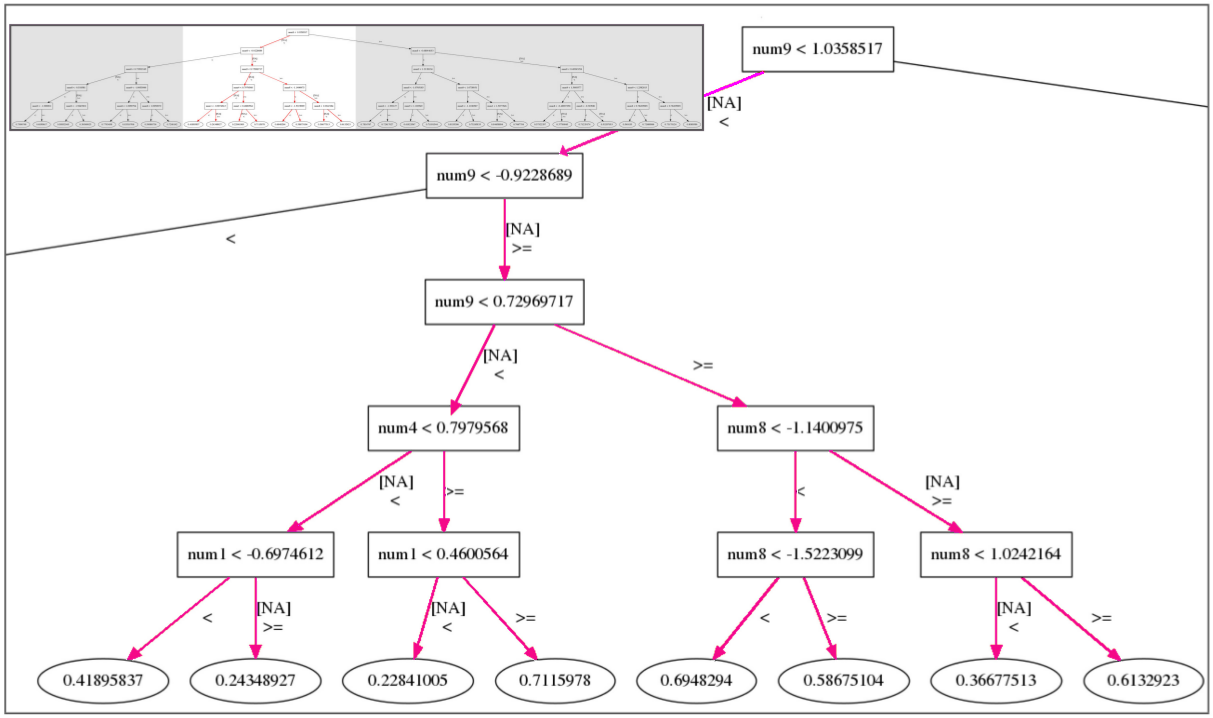
\includegraphics[height=0.6\linewidth, width=.95\linewidth]{../img/figure_3-eps-converted-to.png}\\
  			\tiny{Na\"ive $h_{\text{tree}}$, \textit{a surrogate model}, forms an approximate overall flowchart for the explained model, $g_{\text{GBM}}$.}

			\hspace{5pt}
			\column{.45\textwidth}
  			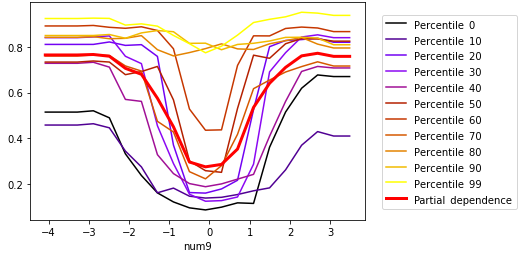
\includegraphics[height=.52\linewidth, width=1.02\linewidth]{../img/figure_4.png}\\
  			\tiny{Partial dependence and ICE curves generated \textit{directly from the explained model}, $g_{\text{GBM}}$.}
  			
  		\end{columns}

	\scriptsize{$h_{\text{tree}}$ displays known interactions in $f = X_{\text{num}1} * X_{\text{num}4} + |X_{\text{num}8}| * X_{\text{num}9}^2$ for $\sim -0.923 < X_{\text{num9}} <  \sim 1.04$. Modeling of the known interaction between $X_{\text{num9}}$ and $X_{\text{num8}}$ in $f$ by $g_{\text{GBM}}$ is also highlighted by the divergence of partial dependence and ICE curves for $\sim -1 < X_{\text{num9}} <  \sim 1$.}

	\end{frame}

	\begin{frame}[t, label={lime}]
	
		\frametitle{\textbf{Example 3.1}: Augment LIME with Direct Explanations}
	
		\begin{columns}
				
			\column{0.5\linewidth}
			\centering			
			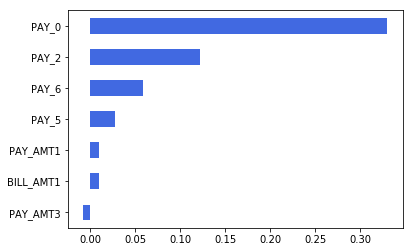
\includegraphics[height=0.6\linewidth, width=.95\linewidth]{../img/shap_blue.png}\\
  			\tiny{Locally accurate Shapley contributions for a high risk individual's probability of default as predicted by a simple decision tree model, $g_{\text{tree}}$. See slide~\ref{dt} for a directed graph representation of $g_{\text{tree}}$}.

			\hspace{5pt}
			\column{0.5\linewidth}
			\begin{table}
				\centering
				\tiny
				\begin{tabular}{ | p{2cm} | p{1.7cm} | }
					\hline
					$h_{\text{GLM}}$\newline Feature & $h_{\text{GLM}}$\newline Coefficient \\ 
					\hline
					\texttt{PAY\_0 == 4} & $0.0009$ \\
					\hline
					\texttt{PAY\_2 == 3} & $0.0065$ \\
					\hline
					\texttt{PAY\_6 == 2} & $0.0036$ \\
					\hline
					\texttt{PAY\_5 == 2} & $-0.0006$ \\
					\hline					
					\texttt{PAY\_AMT1} & $4.8062\mathrm{e}{-07}$ \\
					\hline										
					\texttt{BILL\_AMT1} & $3.4339\mathrm{e}{-08}$ \\
					\hline
					\texttt{PAY\_AMT3} & $-5.867\mathrm{e}{-07}$ \\	
					\hline	
				\end{tabular}	
			\end{table}	
  			\tiny{Coefficients for a local linear interpretable model, $h_{\text{GLM}}$, with an intercept of 0.77 and an $R^2$ of 0.73, trained between the original inputs and predictions of $g_{\text{tree}}$ for a segment of the UCI credit card dataset with late most recent repayment statuses, $\mathbf{X}_{PAY \_ 0 > 1}$}.
  		\end{columns}

	\scriptsize{Because $h_{GLM}$ is relatively well-fit and has a logical intercept, it can be used along with Shapley values to reason about the modeled average behavior for risky customers and to differentiate the behavior of any one specific risky customer from their peers under the model.}

	\end{frame}


%-------------------------------------------------------------------------------
	\section{High Stakes Applications}
%-------------------------------------------------------------------------------

	\subsection*{} % just for progress indicator

	\begin{frame}
	
		\frametitle{4: Use Highly Transparent Mechanisms for \textbf{High Stakes Applications}}
		\vspace{2pt}
		\centering{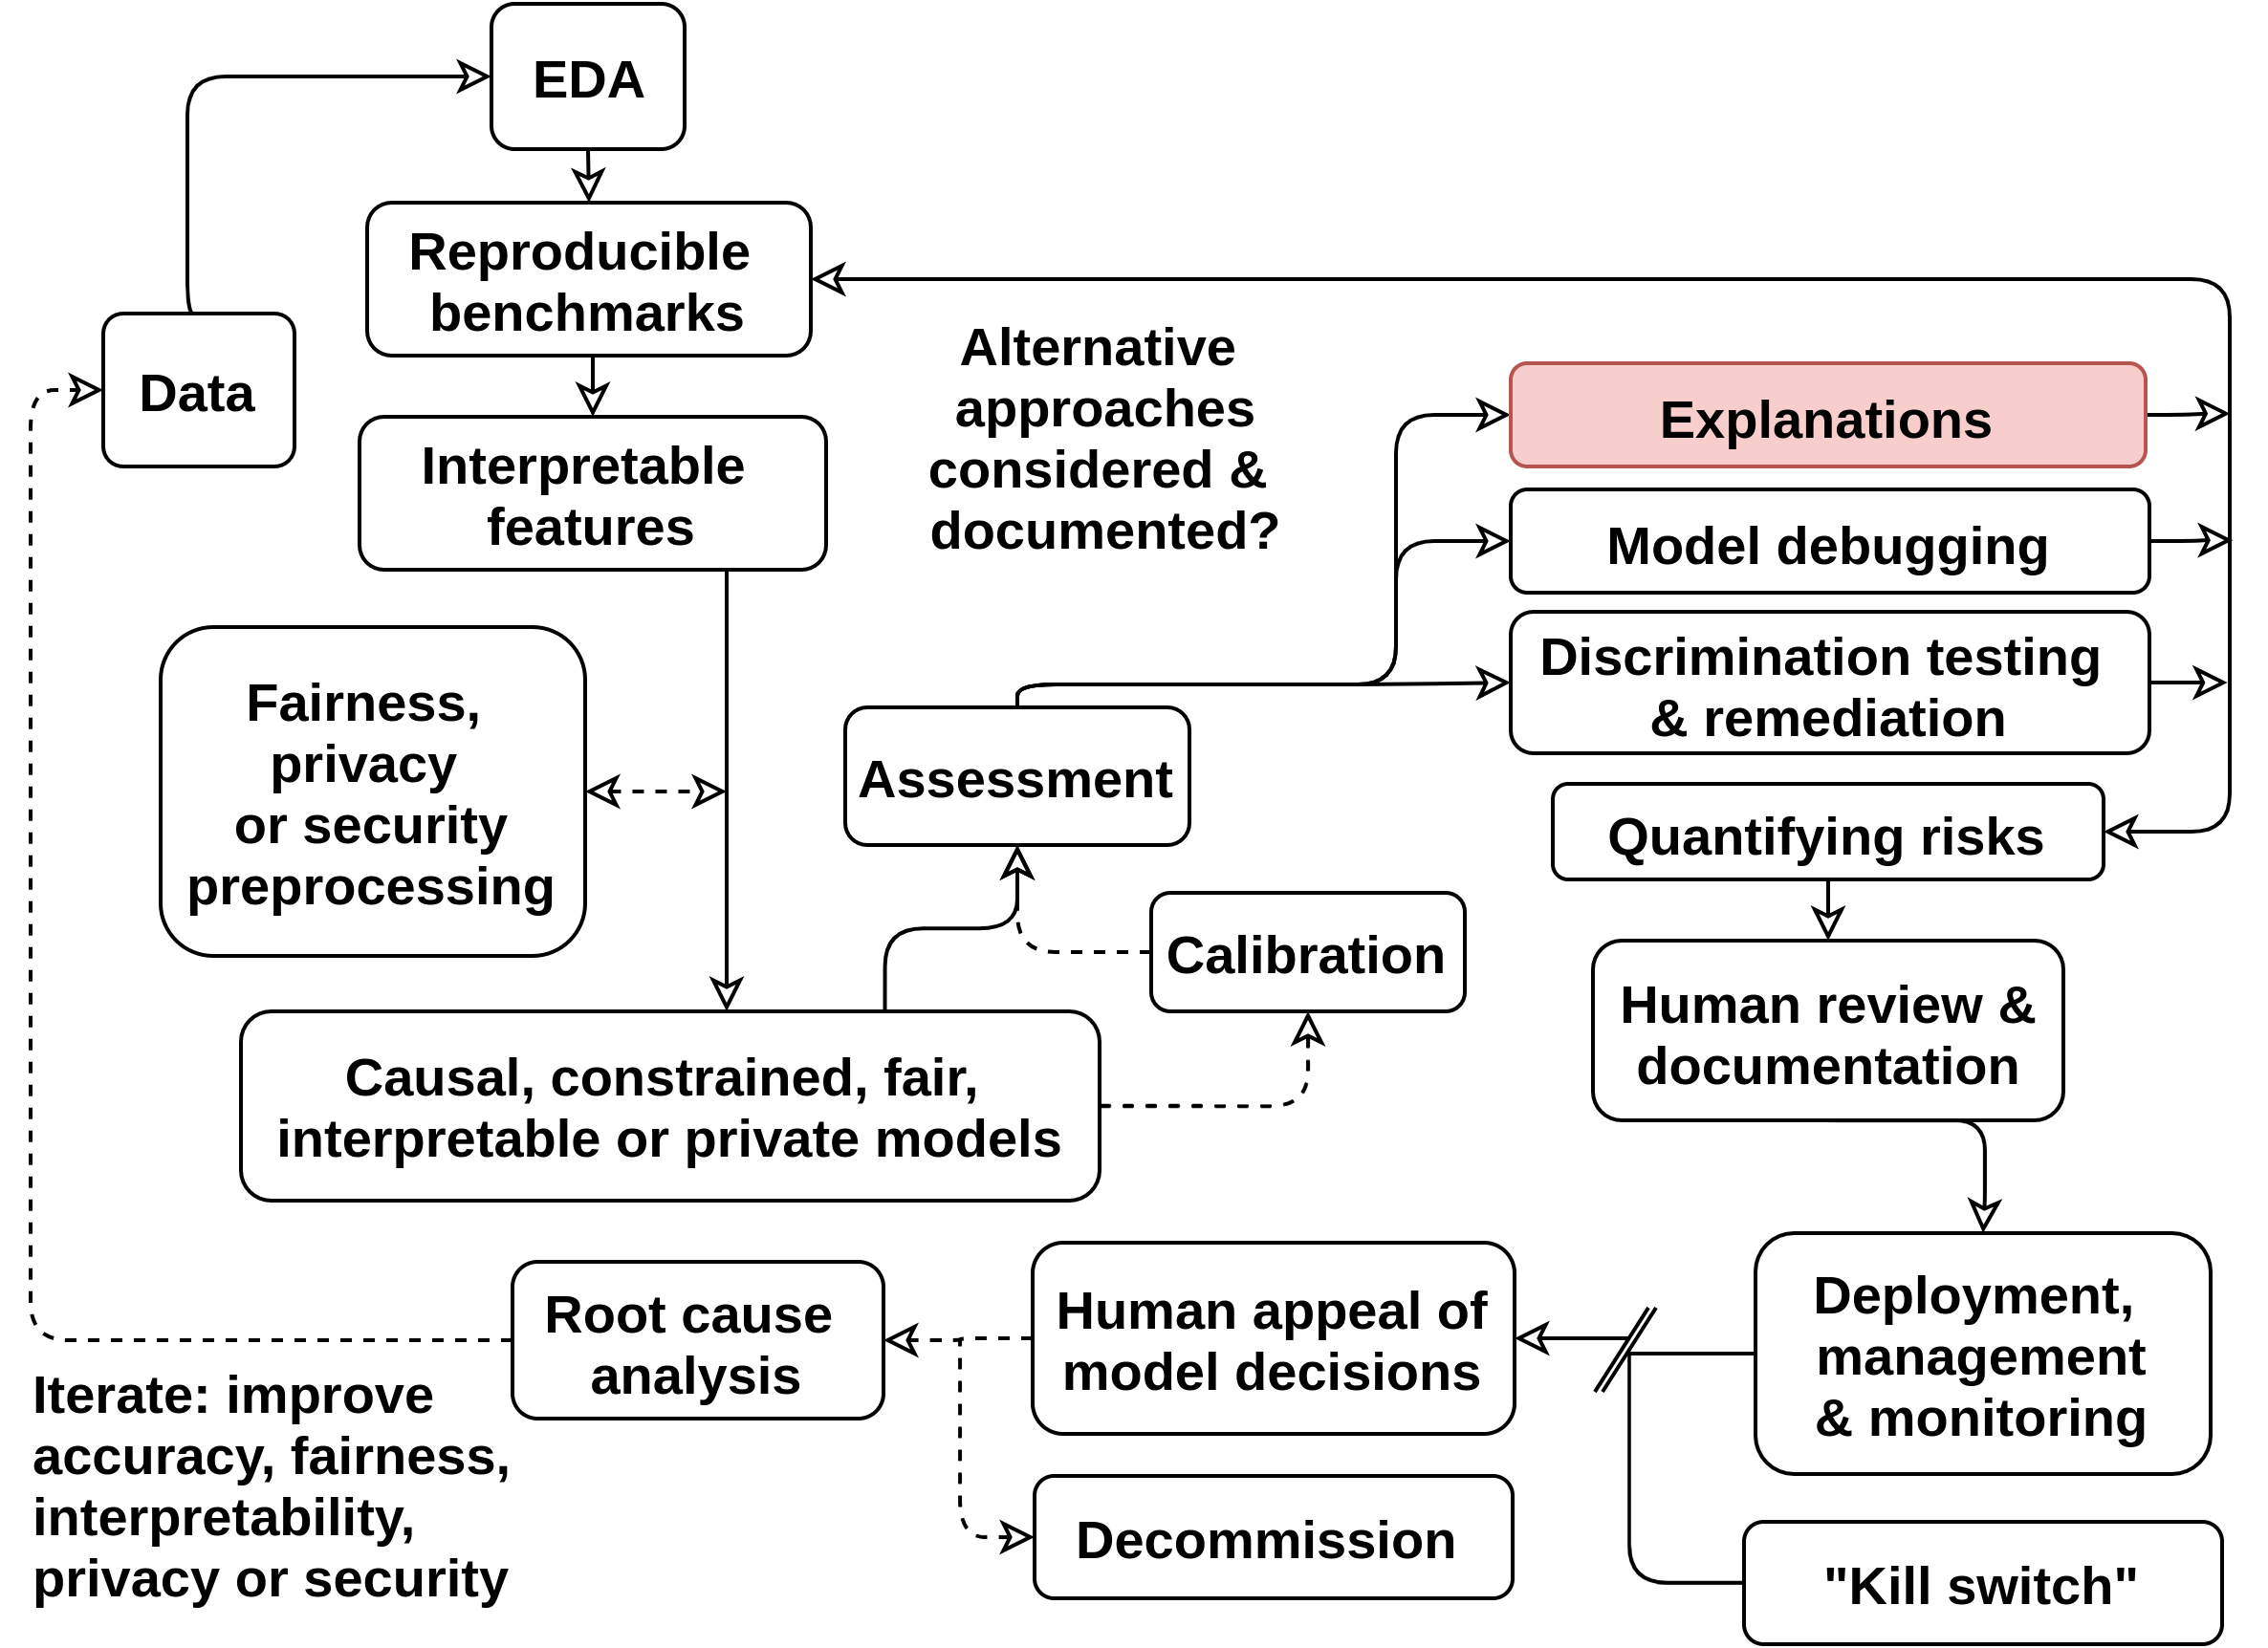
\includegraphics[scale=0.09]{../img/rml_diagram_lec2_hilite.png}}\\
		\vspace{5pt}
		\scriptsize{A diagram of a proposed workflow in which \colorbox{pink}{explanations} are used along with interpretable models, disparate impact analysis and remediation techniques, and other review and appeal mechanisms to create a fair, accountable, and transparent ML system.}
	
	\end{frame}

	\begin{frame}

% XNN

		\frametitle{\normalsize{\textbf{Case 4.1}: Use \textbf{Interpretable Models} for High Stakes Applications (\citet{please_stop})}}
		
		In addition to penalized GLM, decision trees, and conventional rule-based models, many other types of accurate and interpretable models are available today, e.g. ...
		
		\begin{itemize}
			\item \href{https://github.com/microsoft/interpret}{Explainable boosting machine (EBM)}
			\item Monotonic GBM in \href{https://github.com/h2oai/h2o-3}{h2o} or \href{https://github.com/dmlc/xgboost}{XGBoost}
			\item \href{https://cran.r-project.org/web/packages/pre/index.html}{RuleFit} (\citet{rulefit})
			\item \href{https://github.com/ustunb/slim-python}{Super-sparse linear integer model} (SLIM)	(\citet{slim})
			\item Explainable neural network (XNN) (\citet{wf_xnn})
			\item \href{https://cran.r-project.org/web/packages/sbrl/index.html}{Scalable Bayesian rule list} (\citet{sbrl})
		\end{itemize}	

		... use them for human-centered or other high stakes ML applications.\footnote{\tiny{There are shades of interpretability in models. Interpretability is probably not a binary, on-off quality. For instance see Figure 3: \url{https://arxiv.org/pdf/1904.03867.pdf} \cite{molnar2019quantifying}.}}
	
	\end{frame}	

	\begin{frame}[label={dt}]
	
		\frametitle{\normalsize\textbf{Case 4.2}: Explanations and Interpretable Models are \textbf{Not Mutually Exclusive}}
		
		\begin{columns}
				
			\column{0.5\linewidth}
			\centering		
			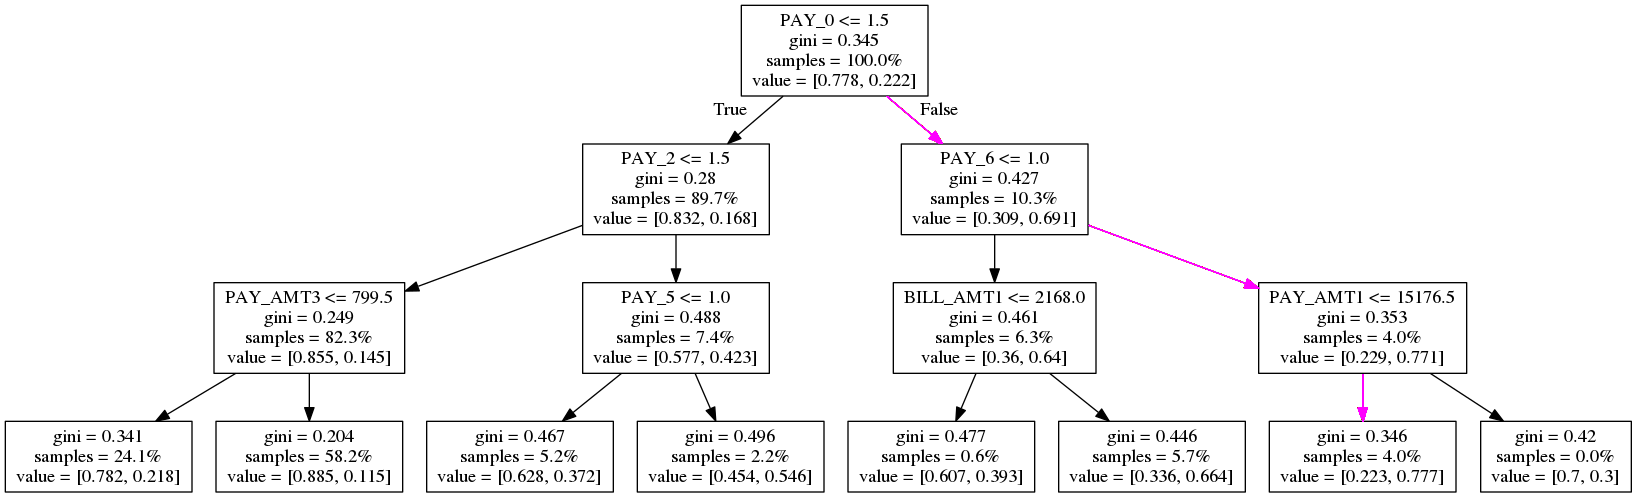
\includegraphics[height=.45\linewidth, width=1.15\linewidth]{../img/dt.png}\\
			\vspace{5pt}
  			\tiny{Simple decision tree, $g_{\text{tree}}$, trained on the UCI credit card data to predict default with validation AUC of 0.74. The decision policy for high risk individuals is highlighted in \textcolor{fuschia}{fuschia}.}

			\hspace{50pt}
			\column{.4\textwidth}
			\centering
			\vspace{2pt}\\
  			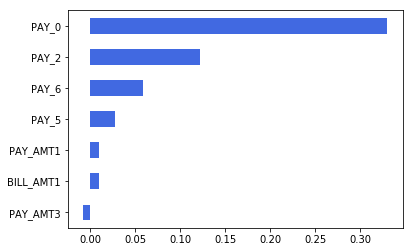
\includegraphics[height=.5\linewidth, width=.8\linewidth]{../img/shap_blue.png}\\
  			\vspace{5pt}
  			\tiny{Locally accurate Shapley contributions for the highlighted individual's probability of default. See slide \ref{lime} for LIMEs for the high risk customers in $g_{\text{tree}}$.}

		\end{columns}
		\vspace{10pt}

	\scriptsize{The Shapley values are helpful because they highlight the local importance of features not on the decision path, which could be underestimated by examining the decision policy alone.}
	
	\end{frame}
	
	\begin{frame}
		
		\frametitle{\textbf{Interlude}: An Ode to the Shapley Value}		
		
		\begin{enumerate}\footnotesize
				
			\item \textbf{In the beginning}: \citefield{shapley1953value}{title}, \citefield{shapley1953value}{year} \cite{shapley1953value}
			\item \textbf{Nobel-worthy contributions}: \citefield{shapley1988shapley}{title}, \citefield{shapley1988shapley}{year} \cite{shapley1988shapley}
			\item \textbf{Shapley regression}: \citefield{lipovetsky2001analysis}{title}, \citefield{lipovetsky2001analysis}{year} \cite{lipovetsky2001analysis}
			\item \textbf{First reference in ML?} \citefield{keinan2004fair}{title}, \citefield{keinan2004fair}{year} \cite{keinan2004fair}
			\item \textbf{Into the ML research mainstream, i.e. JMLR}: \citefield{kononenko2010efficient}{title}, \citefield{kononenko2010efficient}{year} \cite{kononenko2010efficient}
			\item \textbf{Into the real-world data mining workflow ... \textit{finally}}: \citefield{tree_shap}{title}, \citefield{tree_shap}{year}\footnote{\tiny{See \href{https://github.com/h2oai/h2o-3}{h2o}, \href{https://github.com/microsoft/LightGBM}{LightGBM}, or \href{https://github.com/dmlc/xgboost}{XGBoost} for implementation.}} \cite{tree_shap} 
			\item \textbf{Unification}: \citefield{shapley}{title}, \citefield{shapley}{year}\footnote{\tiny{See \href{https://github.com/slundberg/shap}{shap} for implementation.}} \cite{shapley}
				
		\end{enumerate}
			
	\end{frame}
	
	\begin{frame}[t]
	
		\frametitle{\large{\textbf{Case 4.3}: Explanation and Fairness Techniques are \textbf{Not Mutually Exclusive}}}
		
		\begin{table}
			\centering
			\scriptsize
			\begin{tabular}{ | p{1.2cm} | p{1.1cm} | p{1.3cm} | p{1.2cm}| p{1.2cm} | p{1.2cm} | p{1.2cm} | p{1.2cm} | }
				\hline
				& Adverse\newline Impact\newline Disparity & Accuracy Disparity & TPR\newline Disparity & TNR\newline Disparity & FPR\newline Disparity & FNR\newline Disparity \\ 
				\hline	
				\texttt{single} & 0.89 & 1.03 & 0.99 & 1.03 & 0.85 & 1.01 \\
				\hline	
				\texttt{divorced} & 1.01 & 0.93 & 0.81 & 0.96 & \textcolor{fuschia}{1.25} & 1.22 \\
				\hline
				\texttt{other} & \textcolor{fuschia}{0.26} & 1.12 & \textcolor{fuschia}{0.62} & 1.17 & \textcolor{fuschia}{0} & \textcolor{fuschia}{1.44} \\
				\hline	
			\end{tabular}
		\end{table}
		\tiny{Basic group disparity metrics across different marital statuses for monotonically constrained GBM model, $g_{\text{mono}}$, trained on the UCI credit card dataset.	 See slide \ref{no_trust} for global Shapley feature importance for $g_{\text{mono}}$ and slide \ref{not_frontline} for an important note about explanation and fairness techniques.}\\
		\vspace{5pt}\footnotesize
		Many fairness toolkits are available today: \href{https://github.com/dssg/aequitas}{aequitas}, \href{https://github.com/IBM/AIF360}{AIF360}, \href{https://github.com/LASER-UMASS/Themis}{Themis}, \href{https://github.com/cosmicBboy/themis-ml}{themis-ml}.\\
		\vspace{5pt}
		Traditional disparate impact testing tools are best-suited for constrained models because average group metrics cannot reliably identify local instances of discrimination that can occur when using complex, unconstrained models.   
	
	\end{frame}

%-------------------------------------------------------------------------------
		
\section{Acknowledgements} 

	\begin{frame}
	
		\frametitle{Acknowledgments}
		
		Some of the best engineers, researchers, and business leaders in the world!\\
		\vspace{10pt}
		Christoph Molnar, Doug Deloy, Josephine Wang, Kerry O'Shea, Ladislav Ligart, Leland Wilkinson, Mark Chan, Martin Dvorak, Mateusz Dymczyk, Megan and Michal Kurka, Mike Williams, Navdeep Gill, Pramit Choudhary, Przemyslaw Biecek, Sameer Singh, Sri Ambati, Wen Phan, Zac Taschdjian\footnote{\tiny{My world anyway ... and in alphabetical order by first name.}}

	\end{frame}	
			
%-------------------------------------------------------------------------------
% References
%-------------------------------------------------------------------------------


	\begin{frame}[t, allowframebreaks]
	
		\frametitle{References}	
		
			This presentation:\\
			\scriptsize{\url{https://www.github.com/jphall663/kdd_2019}}\\
			\vspace{10pt}
			\normalsize Code examples for this presentation:\\
			\scriptsize{\url{https://www.github.com/jphall663/interpretable_machine_learning_with_python}}\\
			\noindent\scriptsize{\url{https://www.github.com/jphall663/responsible_xai}}\\
			\vspace{10pt}
			\normalsize Associated texts:\\
			\scriptsize{\url{https://arxiv.org/pdf/1810.02909.pdf}}\\
			\noindent\scriptsize{\url{https://arxiv.org/pdf/1906.03533.pdf}}
								
		\framebreak		
		
		\tiny
		\printbibliography
		
	\end{frame}

\end{document}